%% Paper B manuscript skeleton (TRIPOD+AI section order). Tables and figures are generated by the
%% code into tables/ and figures/; do not edit them by hand. Compile with: latexmk -pdf manuscript.tex
\documentclass[11pt,a4paper]{article}
\usepackage[T1]{fontenc}\usepackage[utf8]{inputenc}\usepackage{lmodern}
\usepackage[margin=2.4cm]{geometry}\usepackage{booktabs}\usepackage{graphicx}
\usepackage{amsmath}\usepackage{tabularx}\usepackage{array}\usepackage[hidelinks]{hyperref}
\graphicspath{{figures/}}
\title{How much do leaky splits, missing external validation and missing calibration cost?\\
An empirical companion to a PROBAST+AI/TRIPOD+AI appraisal of machine learning for mental-health prediction}
\author{Aminat Abiola Ajibola \and (co-authors)}
\date{Draft -- \today}
\begin{document}
\maketitle
\begin{abstract}
\textbf{Objective.} [TRIPOD+AI 2] Quantify, on public actigraphy cohorts, the optimism introduced by
three practices that a companion systematic review found to be widespread in machine-learning models
for mental-health prediction: record-wise cross-validation of repeated measures, absence of external
validation, and absence of calibration assessment.
\textbf{Methods.} DEPRESJON (23 depressed, 32 controls), PSYKOSE (22 schizophrenia, shared controls)
and HYPERAKTIV (51 ADHD, 52 clinical controls); one-day windows; majority, logistic regression, random
forest, XGBoost and a 1D-CNN; subject-wise vs record-wise 5-fold CV (E1); train-on-one/test-on-another
without refitting (E2); calibration slope, intercept, Brier, ECE (E3); subject-level BCa bootstrap.
\textbf{Results.} [auto-generated tables; fill after real run].
\textbf{Conclusions.} [..]
\end{abstract}

\section{Introduction}[TRIPOD+AI 3a-b] Motivation from Paper A's proportions; objectives E1--E3.
\section{Methods}
\subsection{Source of data and participants}[4a-b, 5a-b] Cohorts, devices, recruitment (cite source papers); shared control group and its handling.
\subsection{Outcome}[6] Diagnostic group membership per cohort; label semantics per pair.
\subsection{Predictors}[7] Window-level engineered features (list); raw series for the CNN; no demographics.
\subsection{Sample size}[8] Subjects, windows, subject-level EPV (Table~\ref{tab:e2}).
\subsection{Missing data}[9] Validity threshold, median imputation inside the pipeline.
\subsection{Analytical methods}[10a-e, 11, 12] Pipelines, fixed hyper-parameters, splitters, seeds, metrics, bootstrap.
\subsection{Experiments}
\paragraph{E1 leaky splitting.}\paragraph{E2 external validation.}\paragraph{E3 calibration.}
\subsection{Open science}[19-20] Data availability (\texttt{data/README.md}), code availability (repository, tag, SHA), run manifests.
\section{Results}
\subsection{Participants}[21-22]
\subsection{E1}% Auto-generated by mlmh.reporting.tables -- do not edit by hand.
\begin{table}[!htbp]
\centering
\caption{E1: discrimination under subject-wise versus record-wise cross-validation. Cells give the estimate on seed-averaged out-of-fold predictions with subject-level BCa 95\% bootstrap intervals; inflation is the paired record-wise minus subject-wise difference.}
\label{tab:e1}
\footnotesize
\begin{adjustbox}{max width=\linewidth}
\begin{tabular}{llllllll}
\toprule
Cohort & Model & Window AUROC subject-wise & Window AUROC record-wise & Window inflation & Subject AUROC subject-wise & Subject AUROC record-wise & Subject inflation \\
\midrule
depresjon & Majority class & 0.465 [0.292, 0.653] & 0.491 [0.459, 0.528] & 0.026 [-0.147, 0.218] & 0.423 [0.300, 0.551] & 0.427 [0.295, 0.555] & 0.001 [-0.191, 0.202] \\
depresjon & Logistic regression & 0.779 [0.675, 0.861] & 0.845 [0.781, 0.896] & 0.065 [0.024, 0.122] & 0.899 [0.822, 0.969] & 0.965 [0.927, 0.990] & 0.065 [0.011, 0.109] \\
depresjon & Random forest & 0.770 [0.681, 0.848] & 0.877 [0.823, 0.923] & 0.107 [0.058, 0.168] & 0.883 [0.812, 0.948] & 0.977 [0.949, 1.000] & 0.094 [0.041, 0.146] \\
depresjon & XGBoost & 0.764 [0.675, 0.842] & 0.878 [0.830, 0.918] & 0.114 [0.060, 0.181] & 0.874 [0.795, 0.947] & 0.985 [0.964, 1.000] & 0.111 [0.040, 0.175] \\
psykose & Majority class & 0.437 [0.267, 0.632] & 0.500 [0.470, 0.535] & 0.062 [-0.113, 0.241] & 0.419 [0.278, 0.557] & 0.462 [0.331, 0.593] & 0.043 [-0.148, 0.227] \\
psykose & Logistic regression & 0.907 [0.820, 0.942] & 0.927 [0.875, 0.955] & 0.020 [0.006, 0.041] & 0.974 [0.943, 1.000] & 0.994 [0.983, 1.000] & 0.020 [0.000, 0.043] \\
psykose & Random forest & 0.893 [0.798, 0.934] & 0.937 [0.890, 0.962] & 0.044 [0.017, 0.080] & 0.956 [0.913, 0.997] & 0.994 [0.983, 1.000] & 0.038 [0.000, 0.074] \\
psykose & XGBoost & 0.903 [0.810, 0.941] & 0.945 [0.907, 0.969] & 0.042 [0.016, 0.078] & 0.969 [0.935, 1.000] & 0.997 [0.991, 1.000] & 0.028 [0.000, 0.059] \\
hyperaktiv & Majority class & 0.493 [0.355, 0.628] & 0.483 [0.433, 0.533] & -0.010 [-0.170, 0.148] & 0.497 [0.398, 0.597] & 0.443 [0.349, 0.540] & -0.054 [-0.203, 0.106] \\
hyperaktiv & Logistic regression & 0.449 [0.360, 0.535] & 0.579 [0.486, 0.661] & 0.130 [0.095, 0.167] & 0.424 [0.328, 0.519] & 0.601 [0.502, 0.695] & 0.177 [0.131, 0.221] \\
hyperaktiv & Random forest & 0.443 [0.361, 0.534] & 0.612 [0.526, 0.692] & 0.169 [0.135, 0.206] & 0.424 [0.333, 0.518] & 0.641 [0.550, 0.722] & 0.217 [0.177, 0.257] \\
hyperaktiv & XGBoost & 0.442 [0.360, 0.524] & 0.593 [0.518, 0.664] & 0.151 [0.116, 0.186] & 0.438 [0.337, 0.530] & 0.652 [0.555, 0.732] & 0.214 [0.173, 0.261] \\
\bottomrule
\end{tabular}
\end{adjustbox}
\end{table}
% Auto-generated by mlmh.reporting.tables -- do not edit by hand.
\begin{table}[!htbp]
\centering
\caption{E1: window-level discrimination and calibration for every model, cohort and splitting design (mean over seeds).}
\label{tab:e1full}
\footnotesize
\begin{tabular}{llllllllll}
\toprule
Cohort & Model & Split & Accuracy & Macro-F1 & AUROC & Brier & Cal. slope & Cal. intercept & ECE \\
\midrule
depresjon & Majority class & subject-wise & 0.653 & 0.395 & 0.482 & 0.227 & -4.01 & -0.00 & 0.000 \\
depresjon & Majority class & record-wise & 0.653 & 0.395 & 0.499 & 0.227 & 0.29 & 0.00 & 0.000 \\
depresjon & Logistic regression & subject-wise & 0.722 & 0.706 & 0.765 & 0.194 & 0.52 & -0.54 & 0.118 \\
depresjon & Logistic regression & record-wise & 0.761 & 0.750 & 0.840 & 0.163 & 0.90 & -0.62 & 0.095 \\
depresjon & Random forest & subject-wise & 0.724 & 0.679 & 0.762 & 0.185 & 0.69 & 0.01 & 0.061 \\
depresjon & Random forest & record-wise & 0.806 & 0.782 & 0.874 & 0.136 & 1.23 & -0.11 & 0.039 \\
depresjon & XGBoost & subject-wise & 0.722 & 0.676 & 0.745 & 0.202 & 0.43 & 0.29 & 0.123 \\
depresjon & XGBoost & record-wise & 0.802 & 0.776 & 0.872 & 0.137 & 0.82 & 0.07 & 0.039 \\
\bottomrule
\end{tabular}
\end{table}

\begin{figure}[!htbp]\centering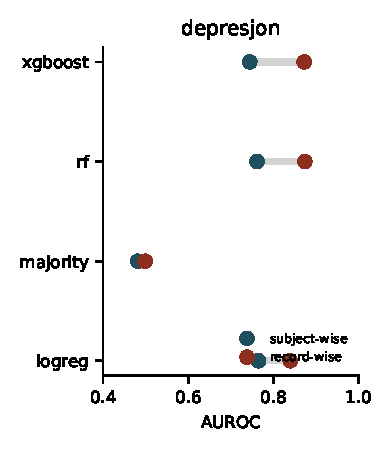
\includegraphics[width=\linewidth]{e1_inflation_auroc.pdf}\caption{E1: AUROC under subject-wise and record-wise CV.}\end{figure}
\subsection{E2}% Auto-generated by mlmh -- do not edit by hand.
\begin{table}[!htbp]
\centering
\caption{E2: internal (subject-wise CV on the training cohort) versus external (unchanged model applied to the second cohort) performance. Window-level estimates, mean over seeds, subject-level BCa 95\% intervals. EPV = minority-class subjects per candidate predictor in the training cohort.}
\label{tab:e2}
\footnotesize
\begin{adjustbox}{max width=\linewidth}
\begin{tabular}{llllllllll}
\toprule
Train $\rightarrow$ Test & Model & EPV & Internal AUROC & External AUROC & $\Delta$ & Int. slope & Ext. slope & Ext. intercept & Ext. Brier \\
\midrule
depresjon $\rightarrow$ psykose & Majority class & 0.6 & 0.475 [0.224, 0.662] & 0.500 [0.500, 0.500] & +0.025 & -4.16 & 0.00 & -0.02 & 0.250 \\
depresjon $\rightarrow$ psykose & Logistic regression & 0.6 & 0.790 [0.701, 0.871] & 0.779 [0.676, 0.847] & -0.011 & 0.66 & 0.50 & 0.06 & 0.193 \\
depresjon $\rightarrow$ psykose & Random forest & 0.6 & 0.730 [0.607, 0.837] & 0.775 [0.688, 0.846] & +0.045 & 0.58 & 0.80 & -0.02 & 0.193 \\
depresjon $\rightarrow$ psykose & XGBoost & 0.6 & 0.716 [0.608, 0.825] & 0.768 [0.678, 0.835] & +0.051 & 0.34 & 0.55 & -0.01 & 0.204 \\
psykose $\rightarrow$ depresjon & Majority class & 0.6 & 0.463 [0.206, 0.601] & 0.500 [0.500, 0.500] & +0.037 & -4.07 & 0.00 & 0.06 & 0.250 \\
psykose $\rightarrow$ depresjon & Logistic regression & 0.6 & 0.881 [0.790, 0.938] & 0.689 [0.564, 0.793] & -0.192 & 0.72 & 0.27 & 1.20 & 0.262 \\
psykose $\rightarrow$ depresjon & Random forest & 0.6 & 0.851 [0.756, 0.926] & 0.728 [0.620, 0.818] & -0.123 & 0.76 & 0.63 & 0.74 & 0.225 \\
psykose $\rightarrow$ depresjon & XGBoost & 0.6 & 0.871 [0.793, 0.936] & 0.670 [0.569, 0.770] & -0.201 & 0.55 & 0.30 & 1.44 & 0.285 \\
depresjon $\rightarrow$ hyperaktiv & Majority class & 0.8 & 0.482 [0.292, 0.653] & 0.500 [0.500, 0.500] & +0.018 & -4.01 & -0.01 & 0.65 & 0.275 \\
depresjon $\rightarrow$ hyperaktiv & Logistic regression & 0.8 & 0.765 [0.675, 0.861] & 0.442 [0.348, 0.532] & -0.323 & 0.52 & -0.16 & -0.42 & 0.350 \\
depresjon $\rightarrow$ hyperaktiv & Random forest & 0.8 & 0.762 [0.681, 0.848] & 0.460 [0.360, 0.557] & -0.301 & 0.69 & -0.15 & 0.33 & 0.317 \\
depresjon $\rightarrow$ hyperaktiv & XGBoost & 0.8 & 0.745 [0.675, 0.842] & 0.459 [0.358, 0.550] & -0.286 & 0.43 & -0.09 & 0.48 & 0.364 \\
\bottomrule
\end{tabular}
\end{adjustbox}
\end{table}

\subsection{E3}% Auto-generated by mlmh.reporting.tables -- do not edit by hand.
\begin{table}[!htbp]
\centering
\caption{E3: calibration alongside discrimination for every model in E1 (subject-wise arm) and E2, plus logistic recalibration of external predictions.}
\label{tab:e3}
\footnotesize
\begin{tabular}{llrrrrr}
\toprule
Exp. & Run & AUROC & Brier & Cal. slope & Cal. intercept & ECE \\
\midrule
E1 & depresjon.logreg.subject\_wise & 0.779 & 0.187 & 0.69 & -0.51 & 0.102 \\
E1 & depresjon.rf.subject\_wise & 0.770 & 0.181 & 0.77 & 0.01 & 0.056 \\
E1 & depresjon.xgboost.subject\_wise & 0.764 & 0.192 & 0.53 & 0.27 & 0.105 \\
\bottomrule
\end{tabular}
\end{table}

\begin{figure}[!htbp]\centering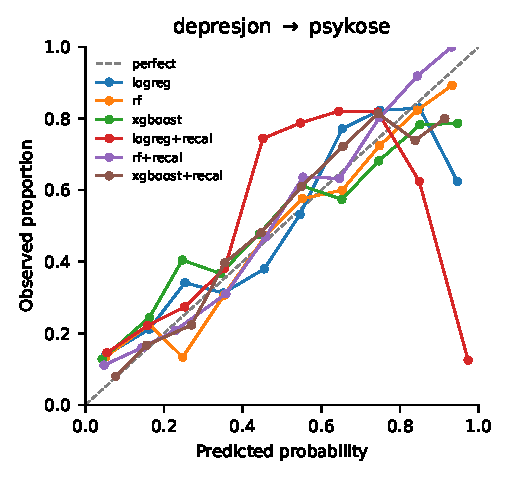
\includegraphics[width=.6\linewidth]{e3_reliability_depresjon_to_psykose.pdf}\caption{E3: reliability curves of external predictions.}\end{figure}
\section{Discussion}[26-27] Interpretation; limitations (n subjects, single device family, label semantics across cohorts, no demographics); implications for Paper A's recommendations.
\section*{Declarations}[16-18] Funding; conflicts; registration (OSF); ethics (secondary use of public de-identified data).
\bibliographystyle{unsrt}
\begin{thebibliography}{9}
\bibitem{garciaceja2018} Garcia-Ceja E, et al. Depresjon: a motor activity database of depression episodes in unipolar and bipolar patients. ACM MMSys 2018.
\bibitem{jakobsen2020} Jakobsen P, et al. PSYKOSE: a motor activity database of patients with schizophrenia. IEEE CBMS 2020.
\bibitem{hicks2021} Hicks SA, et al. HYPERAKTIV: an activity dataset from patients with ADHD. ACM MMSys 2021.
\bibitem{obf2025} Garcia-Ceja E, et al. OBF-Psychiatric, a motor activity dataset of patients diagnosed with major depression, schizophrenia, and ADHD. Sci Data 2025.
\bibitem{collins2024} Collins GS, et al. TRIPOD+AI statement. BMJ 2024;385:e078378.
\bibitem{moons2025} Moons KGM, et al. PROBAST+AI. BMJ 2025.
\bibitem{vancalster2019} Van Calster B, et al. Calibration: the Achilles heel of predictive analytics. BMC Med 2019;17:230.
\end{thebibliography}
\end{document}
